\documentclass[conference]{IEEEtran}
\IEEEoverridecommandlockouts
% The preceding line is only needed to identify funding in the first footnote. If that is unneeded, please comment it out.
\usepackage{cite}
\usepackage{amsmath,amssymb,amsfonts}
\usepackage{graphicx}
\usepackage{textcomp}
\usepackage{xcolor}
\def\BibTeX{{\rm B\kern-.05em{\sc i\kern-.025em b}\kern-.08em
    T\kern-.1667em\lower.7ex\hbox{E}\kern-.125emX}}
\title{
\vspace{1cm}
{
\includegraphics[width=0.15\textwidth]{/storage/emulated/0/FWC1/avr gcc/IMG-20241021-WA0004.jpg} \\ AVR GCC Assignment} }
\author{Sivva Pranaykumar\\ Roll No: FWC22273\\ sivvapranay.s@gmail.com}
 \begin{document}
\maketitle
 \section {ABSTRACT}
A 4-bit priority encoder has inputs D3, D2, D1 and D0 in descending order of priority. The two-bit output AB is generated as 00, 01, 10 and 11 corresponding to inputs D3, D2, D1 and D0, respectively. The Boolean expression of the output bit B is to be implemented.
\section{COMPONENTS}
The required components list is given in Table: I. 

 \begin{table} [htbp]
\centering
\begin{tabular}{| c | c | c |} \hline
Components & Value & Quantity \\\hline
LEDs &  & 1 \\ \hline
Arduino & UNO & 1 \\ \hline
Jumper Wires &  & 10 \\ \hline
Breadboard & & 1 \\ 
\hline
\end{tabular}
\vspace{0.1cm}
\caption{\label{tab:widgets}}
\end{table}
\section{PROCEDURE}
To set up the circuit, power off the Arduino and connect the necessary components: set pin D13 as output (LED connected) and pins D2,D3,D4 and D5 as inputs for D3,D2,D1 and D0 respectively. Connect D2,D3,D4 and D5 to VCC or GND according to the truth table that matches the simplified function. Once everything is set up, power on the Arduino and observe the output based on the truth table.

Pin Configuration: The code initializes the AVR microcontroller by setting the pins connected to D3,D2,D1,D0 as inputs, and the pin connected to the output B as an output.
Reading Inputs: In an infinite loop, the program reads the input values from the corresponding pins.
Boolean Logic Implementation: The code implements the Boolean expression 
$B={\bar{D3}}D2+{\bar{D3}} {\bar{D1}}$. It calculates the value of B based on the priority encoder logic using logical operations.
Output Control: The result of the Boolean logic is used to control the output pin for B. If B=1, the pin is set high, otherwise, it is set low.
\begin{table} [htbp]
\centering
\begin{tabular}{| c | c | c | c | c | c |} \hline
D3& D2& D1& D0& A & B  \\\hline
1 & x & x & x & 0 & 0\\ \hline
0 & 1 & x & x & 0 & 1\\ \hline
0 & 0 & 1 & x & 1 & 0\\ \hline
0 & 0 & 0 & 1 & 1 & 1 \\ \hline

\end{tabular}
\vspace{0.2cm}
\caption{\label{tab:widgets}}
\end{table}

\section{RESULTS}
The program correctly determines the value of B based on the input pins and updates the output pin accordingly. The code operates continuously in a loop to monitor changes in the input signals.https://github.com/Pranaykuma/FWC-1/blob/main/AVR%20GCC/main.c
\begin{figure}[h] 
	\centering 
	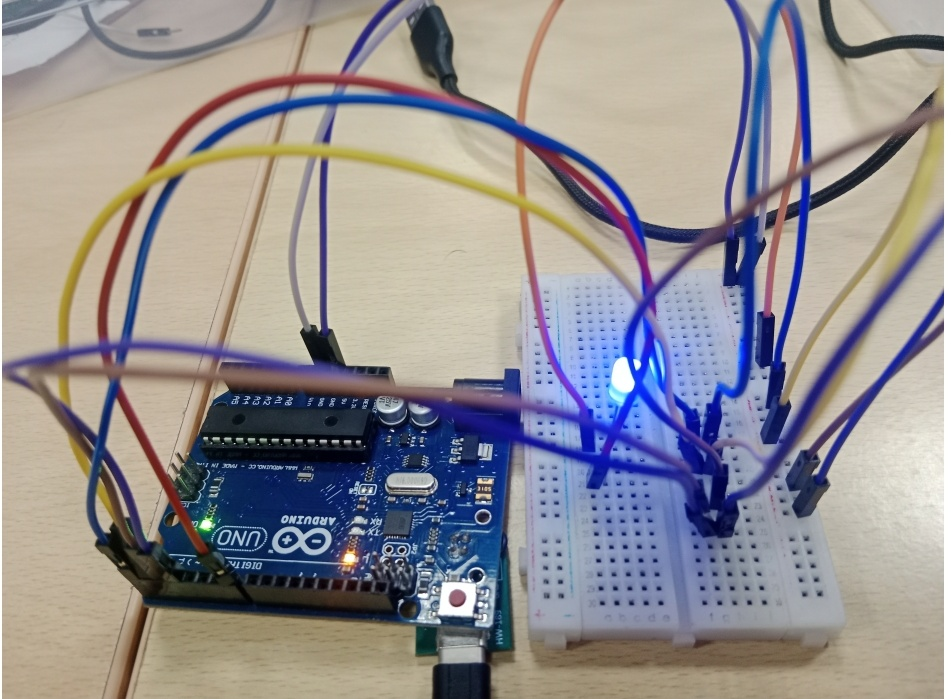
\includegraphics[width=0.4\textwidth]{/storage/emulated/0/FWC1/avr gcc/Screenshot_20241024-130606__01.jpg}
	\caption{\label{fig:Gates}}    
\end{figure}
\section{CONCLUSION}
Encoders play a critical role in a wide range of applications,
offering precise and reliable data about position, speed, and
direction. Therefore, we can design several circuits and can
be implemented with Arduino using Assembly languag
\end{document}
